\chapter{Resultados}
%TODO: introduce lo que se va a hacer en este capítulo

%TODO: organiza en secciones los distintos experimentos.

\section{mIoU}

Para saber qué porcentaje de acierto ha tenido el proceso de segmentación semántica utilizaremos la métrica conocida como \ac{mIoU} \cite{miou-iou}. Esta métrica se basa en hacer la media de la \ac{IoU} de las diferentes etiquetas de clases.

La \ac{IoU} \cite{miou-iou} es la relación de superposición que existe entre la imagen segmentada y la original. Es decir, sirve para dictaminar con cuánta precisión se ha realizado el proceso de \ac{SS}. En las siguientes figuras se puede ver un ejemplo muy práctico:

\begin{figure}[H]
  \centering
  \includegraphics[width=8cm]{Figuras/Iou_1.eps}
  \caption{Imagen Original}
\end{figure}

\begin{figure}[H]
  \centering
  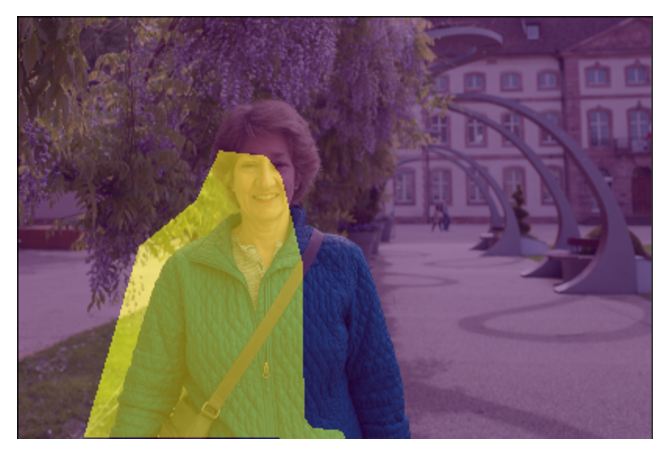
\includegraphics[width=8cm]{Figuras/IoU_2.eps}
  \caption{Predicción}
\end{figure}
%TODO_DONE: yo suelo añadir una sección explicando las métricas, pero no es necesario, si las explicas en cada experimento. Recuerda traer aquí la explicación de la mIOU para evaluar la segmentación semántica.

\section{Evaluación de la segmentación semántica}
...
\section{Evaluación en $ISA^2$}

%TODO hay que añadir una subsección donde se explique el diseño del experimento, es decir, qué se emplea para training, y qué para test, de cada una de las secuencias que forman ISA^2

En la siguiente tabla pasamos a mostrar los resultados tanto de la versión anterior de $ISA^{2}$ \cite{xxxx} como de la desarrollada en este trabajo. Como ya dijimos anteriormente, el \ac{MAE} será la métrica que usaremos para esta tarea, pues indica cuánta precisión ha habido en términos de la estimación de la velocidad.



\begin{table}[H]
\centering
\resizebox{16cm}{!}{
\begin{tabular}{|l|l|l|l|l|l|}\cline{1-6}
& & \multicolumn{2}{|l|}{\textbf{MAE Swiftnet}} & \multicolumn{2}{|l|}{\textbf{MAE DeepLab}} \\ \cline{1-6}
\textbf{Regresión} & \textbf{Nivel de \ac{SPP}} & \textbf{Highway (\%)} & \textbf{Urban (\%)} & \textbf{Highway (\%)} & \textbf{Urban (\%)}\\ \cline{1-6}
\multirow{3}{*}{\textbf{\textit{Linear}}} & 1 & 12.22 & 8.95 & 10.32 & 8.38 \\ \cline{2-6}
& 2 & 13.94 & 9.45 & 11.18 & 8.81 \\ \cline{2-6}
& 3 & 13.39 & \textbf{\textit{11.79}} & 15.5 & \textbf{\textit{10.83}}\\ \cline{1-6}
\multirow{3}{*}{\textbf{\textit{Lasso}}} & 1 & 12.90 & 9.23 & 11.29 & 8.43 \\ \cline{2-6}
 & 2 & 13.80 & 9.40 & 11.7 & 8.62 \\ \cline{2-6}
 & 3 & 13.47 & 10.16 & 10.8 & 9.25\\ \cline{1-6}
\multirow{3}{*}{\textbf{\textit{Boosting Trees}}} & 1 & 13.43 & \textbf{9.83} & 11.35 & \textbf{10.14} \\ \cline{2-6}
 & 2 & 14.97 & \textbf{10.52} & 12.23 & \textbf{10.72}\\ \cline{2-6}
 & 3 & 14.75 & \textbf{10.08} & 10.37 & \textbf{10.12}\\ \cline{1-6}
\multirow{3}{*}{\textbf{\textit{SVR}}} & 1 & 11.13 & \textbf{8.74} & 9.69 & \textbf{9.55} \\ \cline{2-6}
 & 2 & 12.24 & \textbf{8.98} & 9.98 & \textbf{9.09}\\ \cline{2-6}
 & 3 & 12.09 & \textbf{9.60} & 9.78 & \textbf{9.62}\\ \cline{1-6}
\end{tabular}
}
\caption{Tabla de resultados} %TODO: añade más información , sobre qué experimento, incluso comenta el ganador.}
\end{table}

Como se puede apreciar, para cada modelo de \ac{SS} se han segmentado imágenes correspondientes a autovías (o autopistas) y a entornos urbanos. %TODO: da más detalles, donde se entrena, dódne se prueba, se trata de repetir lo del diseño del experimento

Los valores de Swiftnet que aparecen \textbf{resaltados} indican que son mejores que los valores de DeepLab (\textbf{también resaltados}) para esa fila.

Por otro lado, hemos puesto dos valores con \textit{\textbf{este aspecto}} para indicar que, durante la predicción de la velocidad en el sistema de regresión lineal, hemos modificado un parámetro para obtener unos resultados más apropiados; ya que, de otra forma, se obtendrían valores muy lejanos a la realidad. %TODO Te refieres la filtrado? hay que explicarlo, dando detalles y poniendo las gráfica

Como se puede observar, tanto los sistemas \textit{Boosting Trees} como \textit{\ac{SVR}} son mejores con la nueva versión de $ISA^2$ que integra Swiftnet para entornos urbanos, mientras que para las autovías es mejor utilizar el modelo DeepLab. Esto quiere decir que Swiftnet trabaja mejor con entornos en los que se requiere más nivel de detalle y DeepLab, por el contrario, lo realiza mejor en entornos más abiertos.

Cabe destacar que Swiftnet \cite{swiftnet} es un modelo \textbf{Real-Time}, de modo que su implementación es menos que costosa que DeepLab, el cual, por el contrario, necesita de un tiempo de procesamiento demasiado elevado para realizar su función. En concreto \ldots %TODO: añade información de tiempos de procesado de uno y otro, en lo que se refiere a segmentación semántica.

A continuación mostramos algunas figuras con las que podemos ver, de forma gráfica, los resultados de los sistemas de regresión con la \ac{SS} realizada por Swiftnet:

\begin{figure}[H]
  \centering
  \begin{subfigure}[b]{0.45\linewidth}
    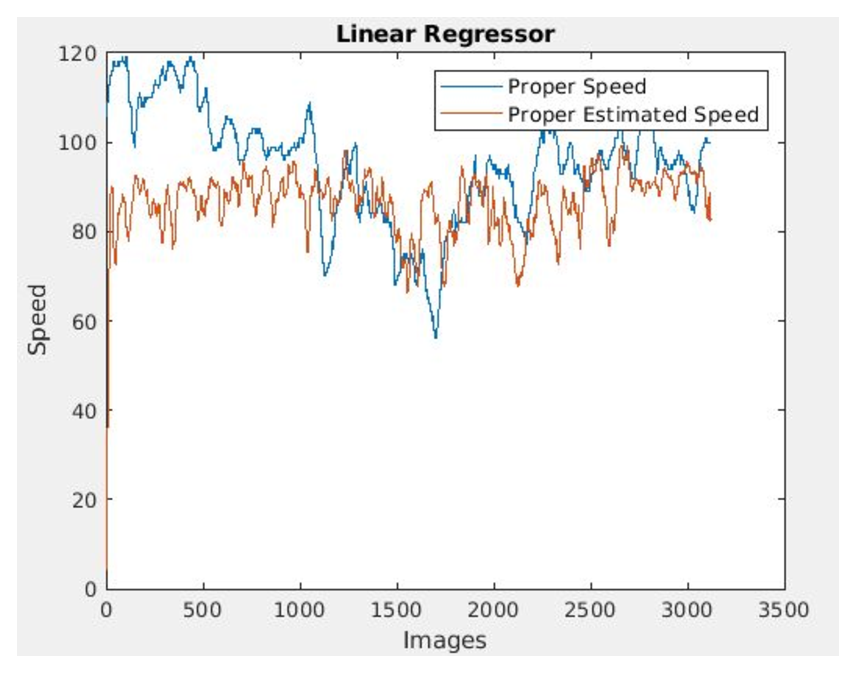
\includegraphics[width=\linewidth]{Figuras/Lineal_Highway(Nivel_1).eps}
    \caption{Highway con Lineal en nivel 1 de \ac{SPP}}
  \end{subfigure}
    \begin{subfigure}[b]{0.425\linewidth}
    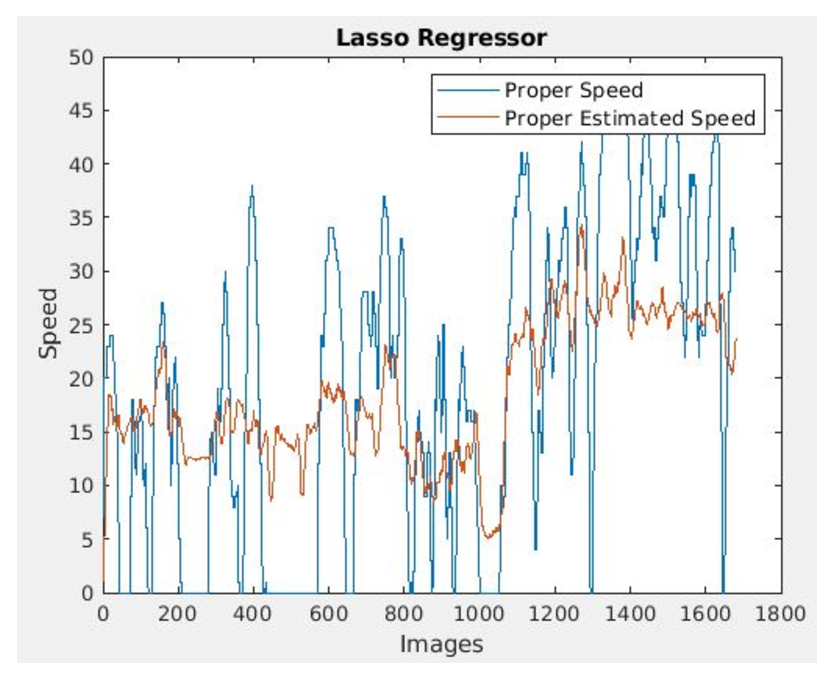
\includegraphics[width=\linewidth]{Figuras/Lasso_Urban(Nivel_1).eps}
    \caption{Urban con Lasso en nivel 1 de \ac{SPP}}
  \end{subfigure}
    \begin{subfigure}[b]{0.45\linewidth}
    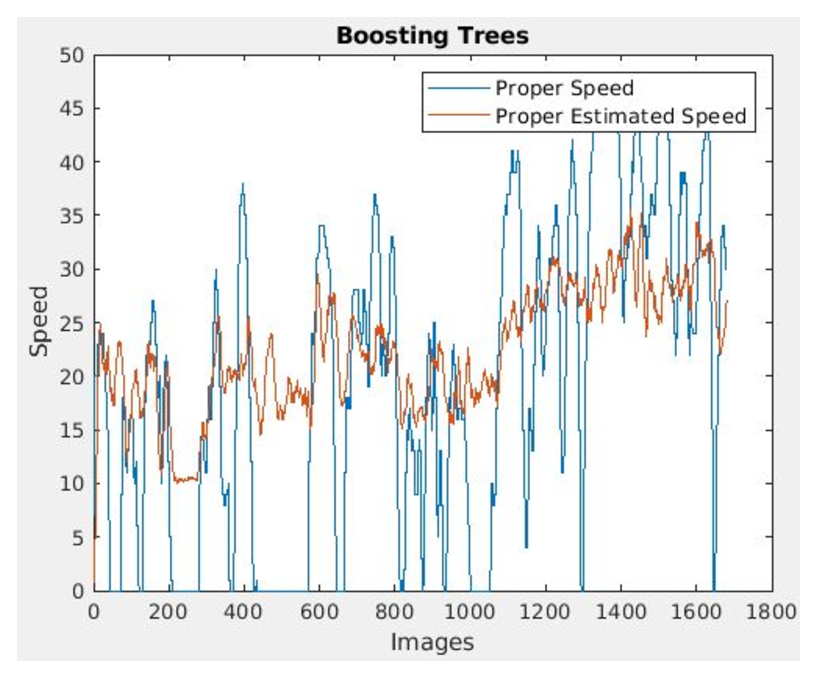
\includegraphics[width=\linewidth]{Figuras/Boosting_Urban(Nivel_1).eps}
    \caption{Urban con Boosting en nivel 1 de \ac{SPP}}
  \end{subfigure}
      \begin{subfigure}[b]{0.45\linewidth}
    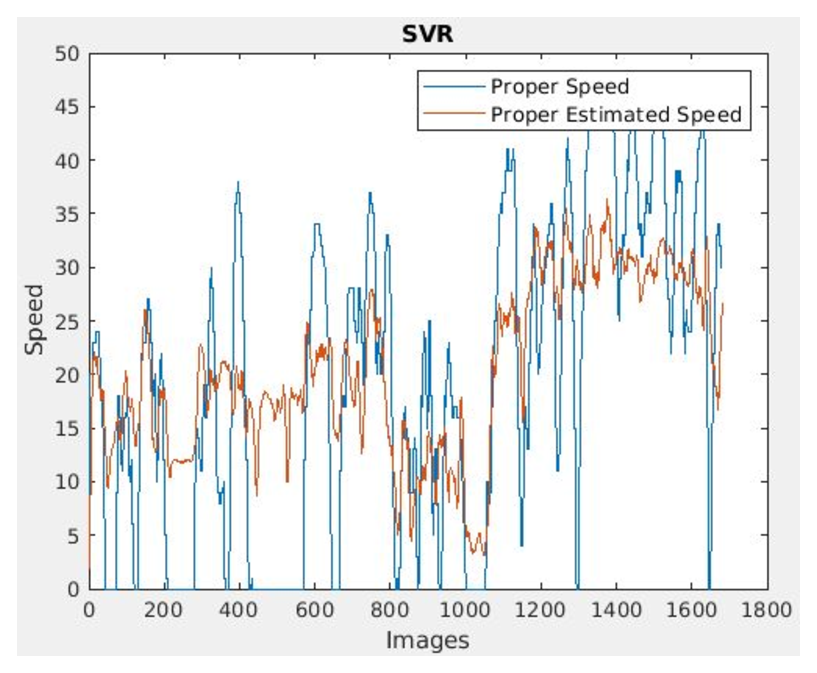
\includegraphics[width=\linewidth]{Figuras/SVR_Urban(Nivel_1).eps}
    \caption{Urban con SVR en nivel 1 de \ac{SPP}}
  \end{subfigure}
  \caption{Resultados gráficos}
\end{figure}

En las figuras, los puntos azules representan la velocidad \textbf{real} a la que debe ir el vehículo en cada imagen, mientras que los puntos rojos representan la velocidad \textbf{estimada} por los sistemas de regresión en cada imagen.

Como se puede observar, hemos escogido, en su mayoría, aquellas figuras en las que los sistemas de regresión han dado mejores resultados, es decir, en entornos urbanos \textbf{(Urban)}. Sin embargo, para contrastar cómo trabaja Swiftnet en autovías hemos decidido poner una figura con esos datos (\textbf{Highway}).

%TODO: faltan muchas cosas. 1) Hay que aclarar que los anteriores resultados, para cada regresor, han sido obtenidos con unos parámetros para el spatial pyramids concretos. Debemos ponerlos. 2) Hay que enriquecer este capítulo con un análisis de la influencia del nivel de la pirámide para cada regresor, así se entenderá porqué hemos puesto los ganadores en la primera tabla. Básicamente una tabla donde comparemos todos con todos los niveles del 1 al 4. 3) falta una sección con los resultados de evaluación en cityscapes en términos de segmentación semántica, donde podamos ver que replicamos los resultados del paper original. Yo pondría esta subsección la primera. 4) Resultados cualitativos: añadir imágenes donde se vea la predicción de la velocidad, y la velocidad anotada, hay que seleccionar las mejores y las peores, y comentarlo. Puedes hacerlo para el modelo ganador nuestro, y creas dos figuras, una con imágenes urbanas y otra con imágenes de autopista. Puedes poner las 4 mejores y las 4 peores. 5) Para el examen conviene que tengas una demo lista en la que podamos ver el sistema funcionando. Lo lanzas contra una carpeta de imágenes y va una a una generando la velocidad, que se guarda en una imagen donde se vea el dato superpuesto, como si fuera un video. Si tienes dudas comentamos. Eso te va a permitir generar un gif a modo de video que te va a quedar muy chulo. 6) Hecho en falta un análsis tiempos de procesado del switnet, para terminar de vender lo de que es tiempo real, vaya. Debes añadirlo.
